\subsection{Разработка функциональных требований}
\label{sec:tech-requirements:functional-requirements}

Функциональные требования (набор сценариев) описывают различное поведение системы в зависимости от входных данных и зависят от типа разрабатываемой системы и
потребностей пользователей.


\textit{\textbf{Модуль управления офисными ресурсами}} должен обеспечивать сотрудникам возможность бронировать рабочие места с учетом их предпочтений и временных интервалов, а также предоставлять менеджерам инструменты для утверждения запросов и автоматической рассадки сотрудников. Все процессы должны быть максимально автоматизированы для минимизации ручного вмешательства. Разрабатываемая система должна предоставлять пользователям осуществлять следующие действия:

\begin{enumerate}
    \item \textit{Создание запроса на бронирование рабочего места}. Система должна предоставлять возможность сотруднику создавать запрос на бронирование рабочего места. Запрос должен включать:
        \begin{itemize}
            \item выбор офиса, этажа, комнаты и конкретного рабочего места;
            \item указание временного интервала бронирования (временное или постоянное);
            \item возможность указания дополнительных предпочтений (например, близость к окну, тихая зона).
        \end{itemize}

    \item \textit{Утверждение (отклонение) запроса на бронирование} рабочего места менеджером или сотрудником с соответствующими правами. После утверждения запроса система должна автоматически обновлять статус рабочего места как занятого.

    \item \textit{Просмотр доступных рабочих мест} в выбранном офисе, этаже или комнате с фильтрацией по различным параметрам (например, доступность, тип рабочего места).

    \item \textit{Автоматическая рассадка сотрудников}. Система должна автоматически распределять сотрудников по рабочим местам на основе заданных параметров (например, предпочтения сотрудников, доступность мест). Возможность ручной корректировки автоматической рассадки менеджером.
\end{enumerate}

Кроме того, в рамках модуля предполагается наличие функциональности для управления оборудованием, которая должна позволять сотрудникам бронировать оборудование, как переносное, так и стационарное, с указанием временного интервала и дополнительных параметров. Менеджеры должны иметь возможность утверждать запросы и контролировать доступность оборудования, обеспечивая его эффективное использование. Это включает в себя реализацию следующих возможностей:

\begin{enumerate}
    \item \textit{Создание запроса на бронирование оборудования}. Запрос должен включать:
        \begin{itemize}
            \item выбор типа оборудования (переносное или непереносное);
            \item указание временного интервала бронирования;
            \item возможность указания дополнительных параметров (например, необходимость доставки оборудования).
        \end{itemize}

    \item \textit{Утверждение (отклонение) запроса на бронирование оборудования} менеджером или сотрудником с соответствующими правами. После утверждения запроса система должна автоматически обновлять статус оборудования как занятого.

    \item \textit{Просмотр доступного оборудования} в выбранной локации с возможностью фильтрации по различным параметрам (например, тип оборудования, доступность).
\end{enumerate}

Также модуль должен предоставлять возможность для автоматизированной генерации отчетов по использованию рабочих мест, оборудования и времени нахождения сотрудников в помещениях, а также предоставлять инструменты для визуализации данных в виде графиков и диаграмм. Это позволит анализировать эффективность использования офисных ресурсов и принимать обоснованные управленческие решения.


\textit{\textbf{Модуль управления сотрудниками}} предполагает наличие функциональности для администрирования сотрудников предприятия. К конкретным требованиям относятся следующие функциональные возможности:

\begin{itemize}
    \item создание, обновление и удаление сотрудников предприятия;
    \item создание, обновление и удаление персональных идентификаторов сотрудников для дальнейшей их интеграции с модулем контроля посещаемости;
    \item автоматизированное ведение журнала истории действий пользователей в системе;
    \item управление иерархией сотрудников предприятия, путем назначения сотрудников к департаментам (отделам), указание профессионального уровня и занимаемой должности.
\end{itemize}


\textit{\textbf{Модуль контроля доступа}} должен интегрироваться с техническими средствами контроля доступа, такими как карты и биометрические системы, для автоматической идентификации сотрудников и управления их доступом в помещения. Учет времени нахождения сотрудников в помещениях и генерация соответствующих отчетов также должны быть реализованы. Это включает в себя наличие следующих возможностей:

\begin{enumerate}
    \item \textit{Управление доступом в помещения}. Система должна предоставлять возможность менеджерам или сотрудникам с соответствующими правами выдавать права доступа в помещения (постоянный или временный доступ) с автоматическим обновлением статуса доступа сотрудника в зависимости от выданных прав.

    \item \textit{Интеграция с техническими средствами контроля доступа}, такими как считыватели персональных карт, биометрические сканеры отпечатков пальцев и системы распознавания лиц. Система должна автоматически идентифицировать сотрудников и управлять их доступом в помещения на основе их роли и прав.

    \item \textit{Отслеживание и учет времени нахождения сотрудников в помещениях} с возможностью генерации различных отчетов по заданным параметрам.
\end{enumerate}


\textit{\textbf{Модуль уведомлений}} предоставляет возможности для автоматизированной отправки уведомлений и рассылок сотрудникам. События, которые вызывают отправку уведомлений, могут вызываться в ручном режиме администраторами системы, или генерироваться автоматически путем выполнения определенных действий в системе, например, утверждении или отклонении запроса на бронирование, выпуск нового персонального идентификатора и тд.

Схема взаимодействия модулей системы приведена на рис.~\ref{fig:tech-requirements:functional-requirements:schema-of-modules}.

\begin{figure}[h]
\centering
    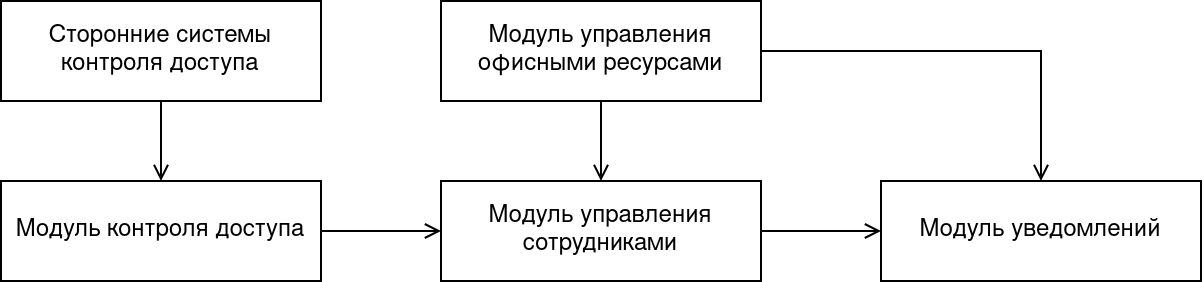
\includegraphics[width=0.9\linewidth]{assets/schema-of-modules.png}
    \caption{Схема взаимодействия модулей системы}
    \label{fig:tech-requirements:functional-requirements:schema-of-modules}
\end{figure}
